% --
% Speech Commands dataset

\subsection{Speech Commands Dataset}\label{sec:exp_dataset_speech_cmd}
The Speech Command Dataset \cite{warden2018} is a very diverse dataset consisting of over thousands of different speakers. This dataset is by any means no clean dataset recorded by professionals, if anything it is the opposite. 
The audio files are not normalized, there are samples with inconsistent sample numbers and some examples are prone with too much noise or even noise only.
And its still great, because there is no need for a perfect dataset and one can be happy that there exists one with this amount of diversity and free of access.
In fact maybe its even better to have an unclean dataset, so that invariances against noise are learnt and do not have be added by hand.
Some examples in raw audio format is shown in \rfig{exp_dataset_wav_grid_c30}.
\begin{figure}[!ht]
  \centering
    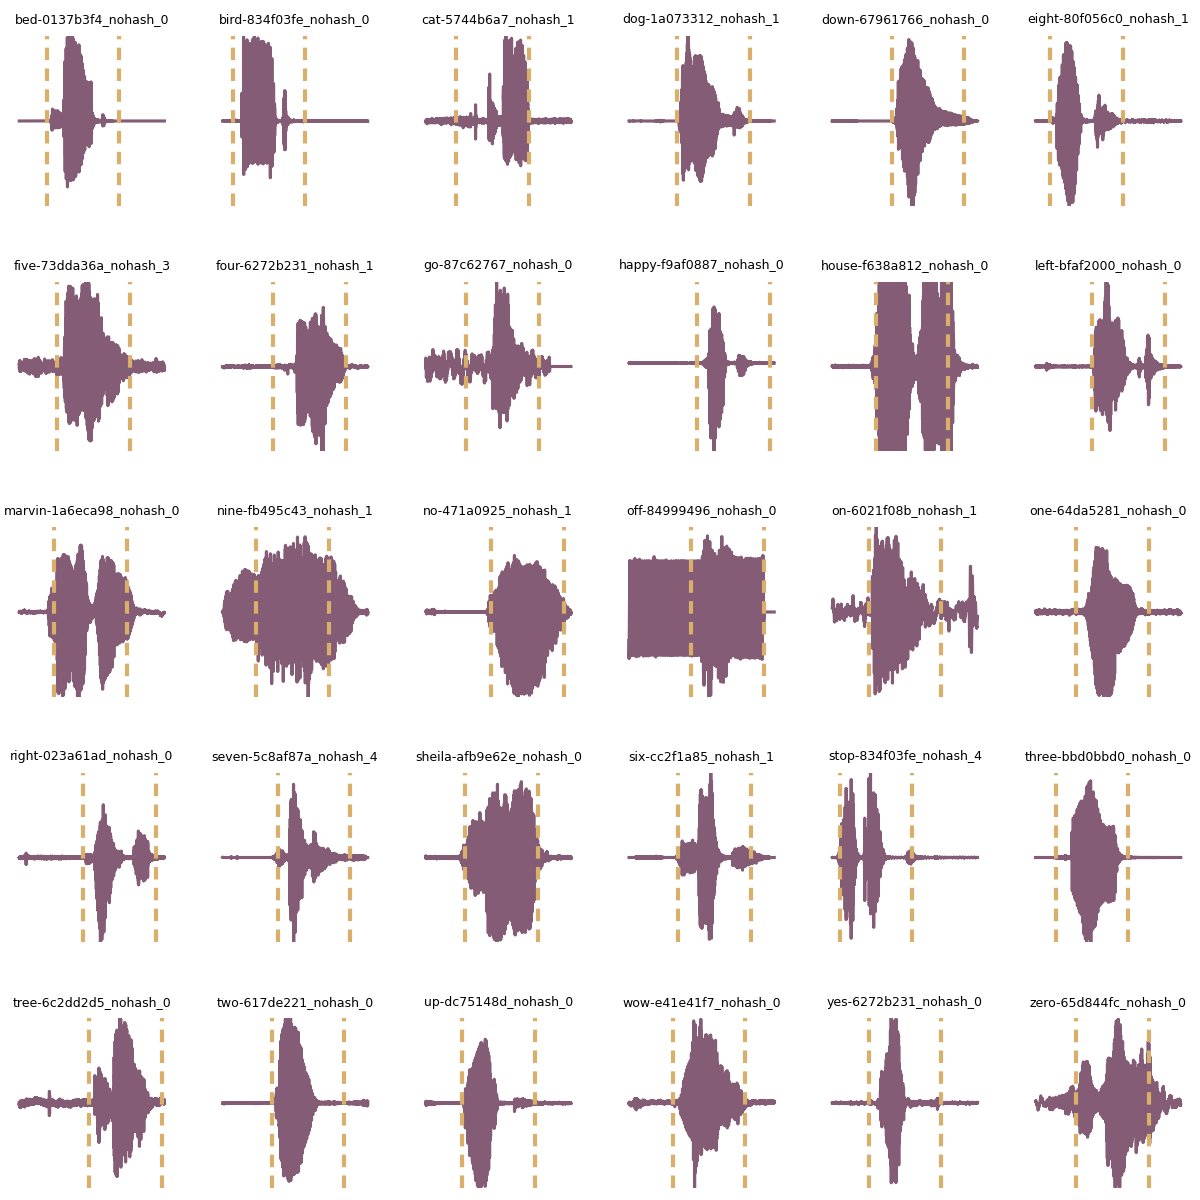
\includegraphics[width=0.65\textwidth]{./5_exp/figs/exp_dataset_wav_grid_c30}
  \caption{Random samples from the Speech Command Dataset, one per class. Pre-processed and normalized raw audio data.}
  \label{fig:exp_dataset_wav_grid_c30}
\end{figure}
\FloatBarrier
\noindent